\section{State Evolution and Loss Between Regions in CeNTREX}
\label{sec:non_adiabatic_transitions}

%%%  NOTES:
% Use coordinate systems $\xi,\upsilon,\zeta$ in comoving frame; X,Y,Z in interaction frame; x,y,z in beam frame
% Suggest to set up abbreviations for regions:  RC, SPA, EQL, SPB, MI, SPC, FD
% Consider removing E<50 V/cm region from Fig 2?    
% Need to add plots: a) all states in 0-50 V/cm  b) what happens in range B=0-10/20 G with E = 50 and/or 100 V/cm.
% Change labels in Fig. 11 to match text
%
%The different functional regions of \CENTREX\ require $\Evec$- and $\Bvec$-fields of widely varying magnitude and orientation. Hence, in the spaces between the functional regions, spatially-varying fields will be present. These manifest as time-varying fields in the molecules' rest frame, resulting in unwanted transfer of molecular population from the desired state to undesired states. This loss reduces statistical sensitivity and can lead to systematic errors. For example, if molecular population is lost non-uniformly over the cross section of the molecular beam, an inhomogeneous distribution of molecules will result. When combined with spatial field gradients within the Main Interaction region, this has been observed to cause systematic errors in related experiments \cite{andreev_improved_2018}. Understanding how the relevant quantum states evolve when molecules travel between functional regions is therefore important both in terms of optimizing the statistics and avoiding systematic errors in \CENTREX.

In this Appendix, we explain in some detail how quantum states evolve as they move between the different regions of the \CENTREX\ beamline.  Our discussion centers on the mechanisms that lead to undesired population transfer, and their likely magnitude in \CENTREX.

Unwanted state transfer is most likely to occur when the desired level undergoes an avoided crossing with an undesired level. Such avoided crossings occur in \CENTREX\ when a pair of states are coupled by one mechanism (e.g., hyperfine or Zeeman interactions) while their energy varies due to a separate mechanism (e.g., Stark shifts in varying $\Evec$-fields). 
%Around the avoided level crossing, the approximate quantum numbers of the system change.
A qualitative understanding of when transitions occur at a level crossing can be found via generalization of the Landau-Zener model \cite{wittig_landauzener_2005}.  We consider cases where the system begins in the pure state $\ket{a}$, and the time-varying energy splitting $\Delta(t)$ between $\ket{a}$ and the other state, $\ket{b}$, goes through 0. Here $\Delta(t)$ refers to the energy splitting when neglecting terms in the Hamiltonian that couple these states, $\mathcal{H}_\text{I}$. The nonzero coupling between the two states, with strength $\hbar\Omega = \bra{a}\mathcal{H}_\text{I}\ket{b} $, leads to an avoided crossing (Fig.~\ref{fig:LZ_energy_diagram}).
\begin{figure}
	\centering
	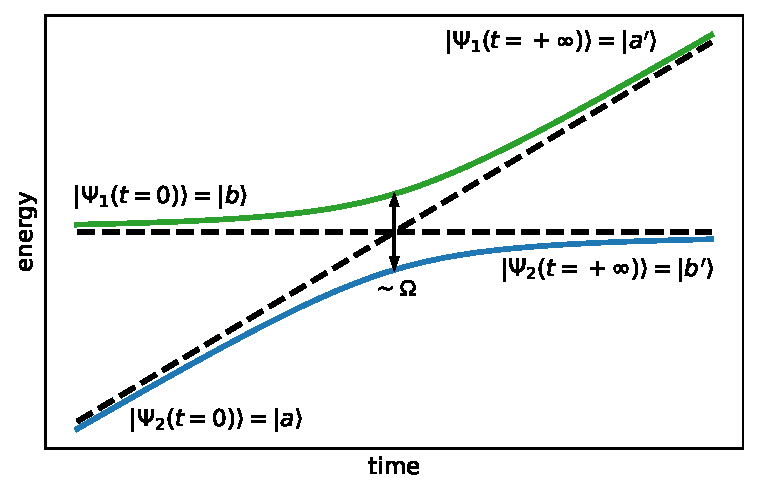
\includegraphics[width=0.48\textwidth,unit=1mm]{figs/matplotlib/lz_energy_diagram.pdf}
	\caption{Energy level diagram for a two-level system with an avoided crossing. Black dashed lines show the energies when $\mathcal{H}_\text{I} = 0$; solid lines show energies in the presence of nonzero coupling strength $\hbar\Omega$. Adiabatic (diabatic) evolution corresponds to initial population in one state remaining on the solid (dashed) lines as the system evolves through the avoided crossing.}
	\label{fig:LZ_energy_diagram}
\end{figure}

Since the character (i.e., good quantum numbers) of each state can be markedly different on either side of an avoided crossing, we label the upper (lower) state after the crossing as $\ket{a'}$ ($\ket{b'}$).  
The state of the system after the avoided crossing is governed by the parameter $\Gamma = \Omega^2/(d\Delta/dt)$. The probability to end in $\ket{b'}$ is large, i.e., the evolution is adiabatic, when $\Gamma \gg 1$. Conversely, the probability to end in $\ket{a'}$ is large, i.e.\ the evolution is sudden, when $\Gamma \ll 1$. In the intermediate range, when $\Gamma\!\sim\! 1$, the final state is generally a superposition of $\ket{a'}$ and $\ket{b'}$, with relative amplitudes that depend critically on the details of the system.

\CENTREX\ is designed so that molecular states evolve either adiabatically, $\Gamma \gg 1$, or suddenly, $\Gamma \ll 1$, through avoided crossings that occur when traversing between functional regions. Thus, the state before and after any such traversal should be deterministically pure. Throughout the experiment, the local $\Evec$-field is always sufficiently large to define a local quantization axis $\hat{\zeta}$, whose direction changes continuously along the molecular trajectory.  In the frame that is co-moving with the molecules, couplings between desired and undesired states arise from hyperfine interactions, Zeeman interactions, or changes in $\Evec$-field direction.  

Earlier experiments using $^{205}$TlF to search for $T$\hyph violation noted severe problems with deterministic state transfer when molecules move from regions of low $\Esca$ to high $\Esca$. This is likely to occur because of the high density of avoided crossings in this transition between regimes \cite{cho1991search,wilkening1984search}.  Hence, throughout the \CENTREX\ apparatus we ensure that $\Esca > 50 \Vcm$, such that only transitions between mid- and high-field regimes are relevant. There are two classes of transition regions where deterministic evolution of pure states is nontrivial in \CENTREX. The first class refers to transitions between the electrostatic lens and State Preparation regions A and B; the second class refers to transitions between the Main Interaction region and State Preparation regions B and C. We discuss each in some detail here.

The $\Esca$-fields in the SPA and SPB regions ($\sim\!100 \Vcm$ maximum) and in the transitions between these and the EQL region ($\sim\!50 \Vcm$ minimum) lie in the mid-field regime; in the EQL region, $\Esca \sim \hbox{10--30} \kVcm$ is in the high-field regime (see Sec.~\ref{sec:TlF_in_E_fields}). In the transition between mid- and high-field regimes, several subtle but important effects arise due to the coupling between molecular rotation $\vec{J}$ and nuclear spins $\vec{I}_1$ and $\vec{I}_2$ (described by the terms proportional to $c_1 $ and $c_2$ in Eq.~\ref{eq:hyperfine_hamiltonian}). 
First, in the mid-field regime (see Sec. \ref{sec:TlF_in_E_fields}), the molecular eigenstates are only nominally described by the mid-field basis states $\ket{J,m_J}\ket{\It,m_{\It}}$ (for $m_J=0$). This means that molecules nominally prepared in the desired state $ \ket{J=2, m_J = 0}\ket{\It=0,m_{\It}=0} $, in the SPA region, are actually prepared in an eigenstate $\ket{\psi_{\rm SPA}}$ that has a small admixture of states with $ m_J = \pm 1 $.
For example, when $\Esca \sim 50 \Vcm$, %(the approximate minimum value of $\Esca$ in the regions of interest),
we find
\begin{equation}
    \begin{split}
    	\ket{\psi_{\rm SPA}} \approx{} & \ket{J=2,m_J=0}\ket{\It=0,m_{\It}=0} \label{eq:SPA_ket}\\
        & {}+\eta \ket{J = 2, m_J = 1}\ket{\It=1,m_{\It}=-1} \\
    	 & {}-\eta \ket{J = 2, m_J = -1}\ket{\It=1,m_{\It}=+1},
    \end{split}
\end{equation}
where the mixing coefficient $\eta$ is determined by the strength of the hyperfine interaction compared to the Stark shift between states with different $m_J$: $\eta \approx \hbar\Omega_{\rm hf}/\Delta E_{\rm S} \sim 0.1$.  Here, the nonzero value of $\eta$ arises from the spin-rotation terms in $\mathcal{H}_\text{I}$, which couple states with $\Delta m_J = \pm 1 = -\Delta m_{\It}$. By contrast, in the high-field regime of the EQL, states with different values of $m_J$ are very distant. Hence, here the true eigenstates $\ket{\psi_{\rm EQL}}$, corresponding to the desired states $\ket{\widetilde{J},m_J=0}\ket{\It=0,m_{\It}=0}$, have negligibly small admixtures of states with $m_J\neq 0$ or $\It\neq 0$ (i.e., $\eta \lll 1$).

Second, as a function of $\Esca$ in the transition from mid- to high-field regimes, the (nominal) $\ket{J=2,m_J=0}$ eigenstates with different spin content undergo a few level crossings (Fig.~\ref{fig:spin_state_crossings}).
\begin{figure}
	\centering
	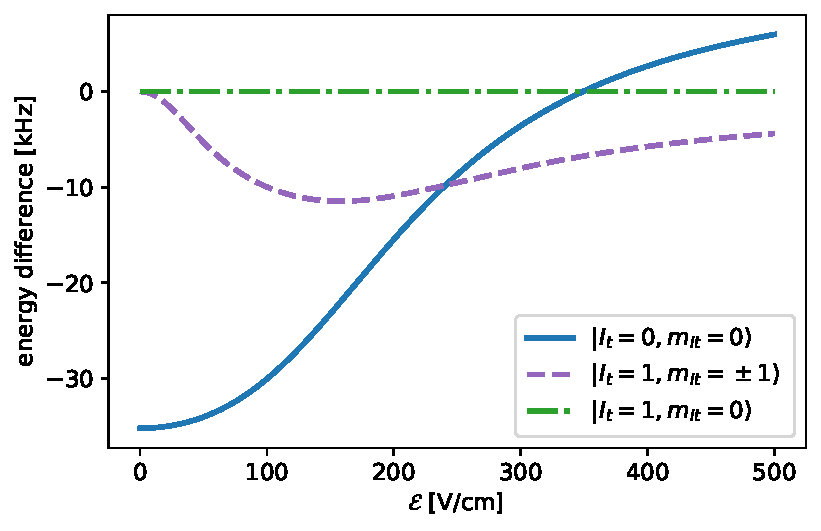
\includegraphics[width=0.48\textwidth,unit=1mm]{figs/matplotlib/spin_state_crossings.pdf}

	\caption{Relative energies of the nuclear spin states within the $J=2, m_J = 0$ manifold, versus $\Esca$-field magnitude (with $\Bsca = 0$). The energy of the $\ket{\It=1, m_{\It} = 0}$ state is defined as the reference energy at every value of $\Esca$. Level crossings occur at $\sim240$ and $350 \Vcm$. If the $\Bvec$-field is non-zero or the $\Evec$-field is rotating, the different spin states will be coupled and the crossings will be avoided.}
	\label{fig:spin_state_crossings}
\end{figure}
This occurs as the spins fully decouple from rotation in any $m_J=0$ rotational state.

Finally, in the  mid-field regime, rotation of the $\Evec$-field can cause transitions between states with (nominally) different nuclear spin configurations. The source of these transitions can be understood qualitatively: in the mid-to-high field regime, $ \vec{J} $ is strongly coupled to $\Evec$ and must reorient appropriately as the electric field rotates. If the rotation of $ \vec{J} $ is too fast for the coupled nuclear spins to follow, their orientation with respect to the quantization axis provided by $ \Evec $ may change so that the spins end up in a different state relative to the local $\hat{\zeta}$-axis.

To describe couplings induced by $\Evec$-field rotation, we follow the approach of Wall et al.\ \cite{wall_nonadiabatic_2010}. We write the Hamiltonian in a co-moving frame with axes $(\xi,\upsilon,\zeta)$, where $\Evec$ defines the local direction of the $\zeta$-axis at all points along the molecular trajectory. In this frame, $\hat{\zeta}$ may point in any direction relative to a set of laboratory-fixed axes, and its direction rotates continuously as the molecules move along their path in the lab. Consider what happens when a molecule moves from the low field in the SPA region to the high field in the EQL region. In the SPA region, $\Evec$ is parallel to the average molecular beam direction, $\hat{Z}$. The quadrupole field is always in the $X-Y$ plane in this frame; here we consider a particular molecular trajectory such that the direction of $\Evec$ inside the lens is along $\hat{X}$. (Analogous arguments hold for other trajectories.)

To keep the $\Evec$-field along $\hat{\zeta}$, we rotate co-moving coordinate system about the laboratory $Y$-axis, by an angle $ \theta(t) = \arctan\left(\frac{\Esca_{\rm EQL}(t)}{\Esca_{\rm SPA}(t)}\right)$. Here, $ \Esca_{\rm EQL}(t) $ is the magnitude of the transverse field due to the EQL, and $ \Esca_{\rm SPA}(t) $ that of the axial field due to the ring electrodes in the SPA region. As the molecule moves between the regions, it will see the electric field rotate as $\Esca_{\rm SPA}$ diminishes and $\Esca_{\rm EQL}$ increases (see Figure~\ref{fig:rotating_electric_field}). The unitary rotation matrix that takes us from the lab frame to the co-moving frame is given by 
\begin{equation}
	U_\text{R}(\theta) = \exp(-i\theta (t) \vec{F}\cdot\hat{Y}),
\end{equation}
where $\vec{F} = \vec{J} + \vec{I}_1 + \vec{I}_2$ is the total angular momentum. The time-evolution in this rotated frame is given by
\begin{equation}
i\hbar\frac{d\ket\psi_\text{R}}{dt} = \mathcal{H}_\text{eff}\ket\psi_\text{R} = 
\left(U_\text{R}^\dagger \mathcal{H} U_\text{R} - i\hbar U_\text{R}^\dagger\frac{dU_\text{R}}{dt}\right)\ket{\psi_\text{R}},
\end{equation}
where $\mathcal{H}$ is the Hamiltonian in the lab frame and $\ket{\psi_\text{R}}$ is the state vector in the rotated frame. The term $U_\text{R}^\dagger \mathcal{H} U_\text{R}$ is the usual Hamiltonian for TlF with a time-varying but non-rotating $\Evec$-field along $\hat{\zeta}$. The other term, $U_\text{R}^\dagger\frac{dU_\text{R}}{dt}$, contains the effects due to the rotation of $\Evec$. This term can be written as
\begin{equation}
\mathcal{H}_\text{int}^\text{(eff)} = - i\hbar U_\text{R}^\dagger\frac{dU_\text{R}}{dt} =  -\hbar\left(J_Y+I_{1,Y}+I_{2,Y}\right)\frac{d\theta}{dt}.
\end{equation}

Due to the spin-rotation interaction, the matrix elements of $J_Y$ between $\ket{\psi_{\rm SPA}}$ and the undesired spin triplet states, nominally $\ket{J=2, m_J = 0}\ket{\It=1,m_{\It}=\mp 1}$, are non-zero; their magnitude is $\Omega \sim \eta \frac{d\theta}{dt}$, where $\eta$ is the mixing coefficient from Eq.~\ref{eq:SPA_ket}. Due to this off-diagonal coupling, the level crossings in Fig.~\ref{fig:spin_state_crossings} become avoided crossings. Hence, fully adiabatic evolution here would result in our desired $\It=0$ state evolving into an undesired $\It=1$ state, as shown in Fig.~\ref{fig:LZ_energy_diagram}. Instead, here we want the state evolution to be sudden/fully diabatic to maintain $\It=0$. To avoid population loss, we thus require $ d\Delta/dt \gg \eta^2 \dot{\theta}^2 $. This condition only needs to be fulfilled when the coupled levels are close in energy, i.e.\ when $\Esca \approx 200-400 \Vcm$ (see Fig.~\ref{fig:spin_state_crossings}). This is achieved in practice by allowing $\Esca_{\rm SPA}$ to decay to $ \approx 50 \Vcm $ before $\Esca_{\rm EQL}$ starts to rapidly increase. The $\Evec$-field is then almost entirely in the transverse direction, i.e., not rotating quickly, by the time the level-crossing occurs (Fig.~\ref{fig:rotating_electric_field}).
\begin{figure}
	\centering
	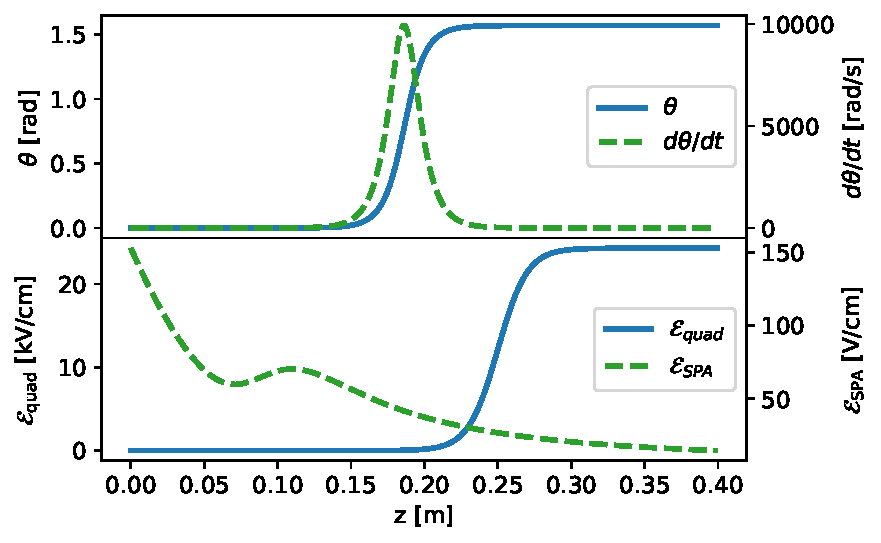
\includegraphics[width=0.48\textwidth,unit=1mm]{figs/matplotlib/rotating_electric_field.pdf}
	\caption{\textbf{Top:} Angle $\theta$ between the $\Evec$-field direction $\hat{\zeta}$ and the lab frame $Z$-axis, and its rate of change over time $d\theta/dt$, for a molecule with typical velocity $\vec{v} = v_Z\hat{Z}$ and $v_Z = 184 \;\mathrm{m/s}$, vs $Z$-position. \textbf{Bottom:} The magnitudes of the $\Esca$-fields in the transition region between the SPL and EQL regions, as a function of $Z$-position. The field due to the SPA region electrodes, $\Evec_\text{SPA}$, is along the length of the apparatus ($Z$); the direction of the field due to the lens electrodes, $\Evec_\text{EQL}$, is taken to be along $X$ in the lab frame. }
	\label{fig:rotating_electric_field}
\end{figure}

We note in passing that the axial-to-transverse field configuration in \CENTREX\ has not been used in previous $^{205}$TlF experiments.  If only transverse fields are used, inevitably some large fraction of molecular trajectories travel through a position where $\Esca=0$ and undesired transitions are strong.  Our approach mimics that of Ref.~\cite{WoodWiemanParity1997}, but using $\Evec$ rather than $\Bvec$ as the quantizing field.

Magnetic fields can also couple the desired $\It=0$, $m_{\It} = 0$ state to $\It=1$ states with $m_{\It}=0$ ($m_{\It} = \pm 1$) when $\Bsca_Z \neq 0$ ($\Bsca_{X,Y} \neq 0$).  To reduce this effect, in \CENTREX\ we will apply shim coils to cancel typical ambient lab fields in the regions of transition into and out of the EQL region. With cancellation by a factor of $\gtrsim 10$, such that $\Bsca \lesssim 0.05\mG$, the Zeeman coupling strengths are in the range $\Omega_Z\lesssim 0.1\kHz$. When the condition needed to avoid transitions from $\Evec$-rotation given above are satisfied, the rate of change of the level splittings as molecules enter the very strong $\Esca$-field of the lens, $d\Delta/dt$, is sufficiently large compared to $\Omega_Z$ such that the evolution is fully diabatic. Numerical simulations indicate a loss of $<1\%$ along any molecular trajectory. Hence, under these conditions the quantum numbers $\It=0,m_{\It}=0$ are preserved as molecules enter and exit the EQL region.

The transition from the EQL region to SPB region is mostly similar to the transition from the SPA region to the EQL region. The primary difference is the requirement in the SPB region to have a uniform electric field $\Evec_{\rm SPB} = \Esca_{\rm SPB} \hat{z}$, along with a substantial magnetic field, $\Bvec_{\rm SPB} = \Bsca_{\rm SPB}\hat{z}$, where $\Bsca_{\rm SPB} \approx \hbox{10--20}\gauss$. Here, we are describing fields in the $(x,y,z)$ ``interaction region'' coordinate system. These fields can be reached by first diabatically rotating from the large transverse lens field $\Evec_{\rm EQL}$ to a weak axial field $\Evec \parallel \hat{Z}$, then adiabatically rotating into the uniform transverse field $\Evec_{\rm SPB} \parallel \hat{z}$. Throughout the second $\Evec$ rotation, $\Esca$ remains in the range $\hbox{50--100} \Vcm$ while $\Bsca_z$ slowly rises, from its initial value of (nominally) zero to $\Bsca_{\rm SPB}$. Though the details remain to be worked out, this scheme should ensure deterministic population of the desired state in the EQL--SPB transition.

The last class of traversals in \CENTREX\ occurs between the SPB and MI regions (or, similarly aside from the reversed sequence, the MI and SPC regions).  Here, the $\Bsca$-field must transform from $\Bsca_{\rm SPB}$ to zero, and the $\Evec$-field can remain in the same $\hat{z}$ direction but must make the transition from low- to high-field regimes.  This can again be accomplished by adiabatically ramping $\Bsca$ to zero while maintaining $\Esca \approx \hbox{50--100} \Vcm$ along $\hat{z}$.  Then, a sudden rise to $\Esca \gg 500 \Vcm$ will maintain the spin quantum numbers for molecules coming into/out of the MI region. During these traversals, there is a possibility of undesired transitions between different nuclear spin states, if the $\Bvec$-field is not fully parallel to the $\Evec$-field. Whether or not these transitions are likely to pose a problem, and if so how to mitigate them, is currently being investigated. We note that in prior experiments with TlF \cite{wilkening1984search,cho1991tight}, this issue was appreciated but not fully under control.
                       
While keeping track of state evolution across level crossings may appear daunting, it is analogous to even more complex schemes that have been applied efficiently in other molecular systems \cite{langheckerdenschlag2008}. We believe that our detailed understanding of and control over these issues will be necessary to understand and minimize systematic errors in \CENTREX.
